\chapter{Factoring Techniques}

Factor each completely.

\begin{multicols}{4}
\begin{enumerate}
	\item $x^2 + 2x - 15$
	\item $a^2-15a+56$
	\item $8x^2+10x+3$
	\item $w^2+w-12$
\end{enumerate}	\setcounter{Review}{\value{enumi}}
\end{multicols}
\begin{multicols}{4}
\begin{enumerate}	\setcounter{enumi}{\value{Review}}
	\item $5b^2-9b-2$
	\item $12x^2+40x-7$
	\item $4x^2-4x-24$
    \item $18t^2-9t-5$
\end{enumerate}	\setcounter{Review}{\value{enumi}}
\end{multicols}
\begin{multicols}{4}
\begin{enumerate}	\setcounter{enumi}{\value{Review}}
	\item $6a^2 + 23a + 21$
	\item $x^2-12x+36$
    \item $9x^2-1$
    \item $4x^2+4x+1$
\end{enumerate}	\setcounter{Review}{\value{enumi}}
\end{multicols}
\begin{multicols}{4}
\begin{enumerate}	\setcounter{enumi}{\value{Review}}
	\item $x^3-x^2-2x$
	\item $6x^2-32x+10$
	\item $2x^3-9x^2-51x-40$
	\item $2x^3+3x^2-3x-2$
\end{enumerate}	\setcounter{Review}{\value{enumi}}
\end{multicols}
\begin{multicols}{4}
\begin{enumerate}	\setcounter{enumi}{\value{Review}}
	\item $4x^3+3x^2-42x+40$
	\item $6x^3-27x^2-168x$
\end{enumerate}	\setcounter{Review}{\value{enumi}}
\end{multicols}

The graph of a factorable expression is shown below. If the expression is in lowest terms (i.e. there is no number in front of all of the parentheses when it is factored) and contains integer coefficients, write the factored form of the expression.
\begin{multicols}{2}
\begin{enumerate}	\setcounter{enumi}{\value{Review}}
\item \mbox{} \newline\\
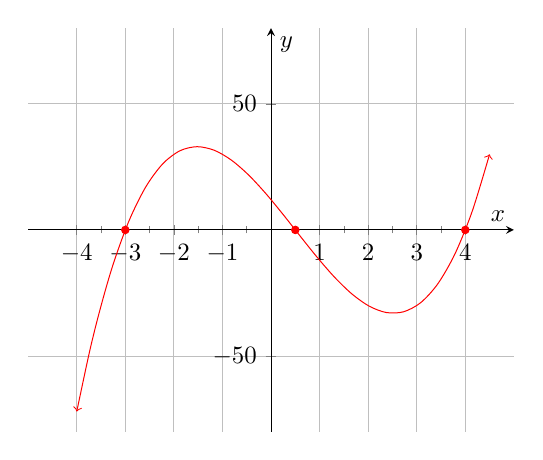
\begin{tikzpicture}[scale=0.9]
\begin{axis}[
axis lines=center, xmin = -5, xmax = 5, ymin=-80, ymax=80,
xtick = {-4,-3,...,4}, minor x tick num = 1, grid=major,
xlabel = $x$, ylabel=$y$]
\addplot [<->, smooth, red, domain=-4:4.5] {2*x^3-3*x^2-23*x+12};
\addplot [red, mark=*, only marks, mark size = 1.5] coordinates {(-3,0) (0.5,0) (4,0)};
\end{axis}
\end{tikzpicture}
\item \mbox{} \newline\\
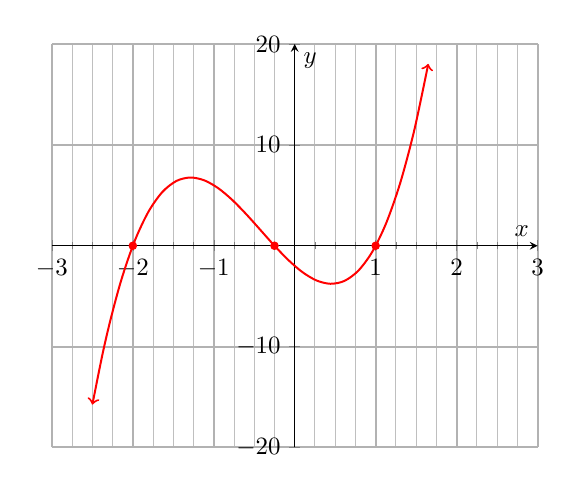
\begin{tikzpicture}[scale=0.9]
\begin{axis}[
axis lines=center, xmin = -3, xmax = 3, ymin=-20, ymax=20,
xtick = {-3,-2,...,3}, minor x tick num = 3, grid=both, major grid style={line width=.8pt,draw=gray!60},
xlabel = $x$, ylabel=$y$]
\addplot [<->, smooth, red, thick, domain=-2.5:1.65] {4*x^3 + 5*x^2 - 7*x - 2};
\addplot [red, mark=*, only marks, mark size = 1.5] coordinates {(-2,0) (-0.25,0) (1,0)};
\end{axis}
\end{tikzpicture}
\end{enumerate}	\setcounter{Review}{\value{enumi}}
\end{multicols}

\begin{multicols}{2}
\begin{enumerate}	\setcounter{enumi}{\value{Review}}
	\item \mbox{} \newline\\
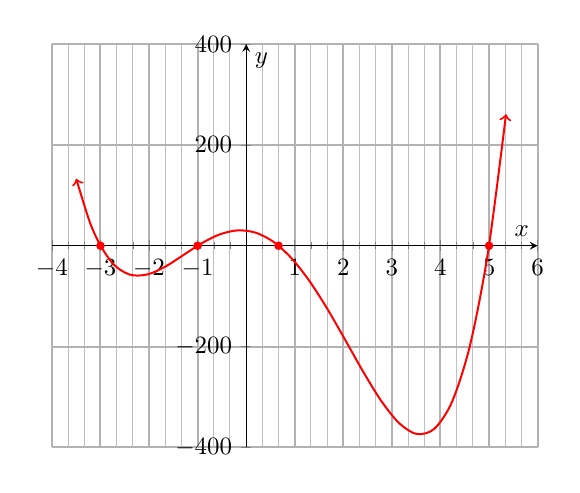
\begin{tikzpicture}[scale=0.9]
\begin{axis}[
axis lines=center, xmin = -4, xmax = 6, ymin=-400, ymax=400,
xtick = {-4,-3,...,6}, minor x tick num = 2, grid=both, major grid style={line width=.8pt,draw=gray!60},
xlabel = $x$, ylabel=$y$]
\addplot [<->, smooth, red, thick, domain=-3.5:5.35] {3*x^4 - 5*x^3 - 49*x^2 - 11*x + 30};
\addplot [red, mark=*, only marks, mark size = 1.5] coordinates {(-3,0) (-1,0) (2/3,0) (5,0)};
\end{axis}
\end{tikzpicture}
\item \mbox{} \newline\\

\end{enumerate}		\setcounter{Review}{\value{enumi}}
\end{multicols}


\newpage

\section{Answer Key}

\begin{enumerate}
	\item $(x+5)(x-3)$
    \item $(a-8)(a-7)$
    \item $(4x+3)(2x+1)$
    \item $(w+4)(w-3)$
	\item $(b-2)(5b+1)$
    \item $(2x+7)(6x-1)$
    \item $4(x-3)(x+2)$
    \item $(3t+1)(6t-5)$
    \item $(3a+7)(2a+3)$
    \item $(x-6)^2$
    \item $(3x-1)(3x+1)$
    \item $(2x+1)^2$
    \item $x(x-2)(x+1)$
    \item $2(3x-1)(x-5)$
    \item $(2x+5)(x+1)(x-8)$
    \item $(x+2)(2x+1)(x-1)$
    \item $(x+4)(4x-5)(x-2)$
    \item $3x(2x+7)(x-8)$
    
    \item $(x+3)(2x-1)(x-4)$
    \item $(x+2)(4x+1)(x-1)$
    \item $(x+3)(x+1)(x-1)(x-5)$
\end{enumerate}